\documentclass[11pt]{article}

\usepackage[letterpaper,margin=0.82in,headheight=14pt]{geometry}
\usepackage[T1]{fontenc}
\usepackage{lmodern}
\usepackage{microtype}
\usepackage{amsmath}
\usepackage{xcolor}
\usepackage{booktabs}
\usepackage{enumitem}
\usepackage{caption}
\usepackage{needspace}
\usepackage{titlesec}
\usepackage{tikz}
\usetikzlibrary{arrows.meta,positioning}
\usepackage{fancyhdr}
\usepackage{hyperref}
\usepackage[backend=biber,style=authoryear,maxcitenames=2,maxbibnames=99,sorting=nyt]{biblatex}
\addbibresource{sources.bib}

\definecolor{ink}{HTML}{203447}
\definecolor{accent}{HTML}{176B82}
\definecolor{topicone}{HTML}{177E89}
\definecolor{topictwo}{HTML}{D38638}
\definecolor{pale}{HTML}{F0F6F8}
\hypersetup{colorlinks=true,linkcolor=accent,citecolor=accent,urlcolor=accent}
\pagestyle{fancy}
\fancyhf{}
\lhead{\small Classical Modeling and Modern Methods}
\rhead{\small Text Mining lecture outline}
\cfoot{\small \thepage}
\setlength{\parindent}{0pt}
\setlength{\parskip}{0.42em}
\setlist[itemize]{leftmargin=1.4em,topsep=2pt,itemsep=1pt,parsep=0pt}
\setlist[enumerate]{leftmargin=1.55em,topsep=2pt,itemsep=1pt,parsep=0pt}
\captionsetup{font=small,labelfont=bf,skip=5pt}
\titlespacing*{\subsection}{0pt}{1.5ex plus 0.3ex}{0.4ex}
\tikzset{
  flowbox/.style={draw=accent,rounded corners=3pt,fill=pale,align=center,
    inner sep=5pt,font=\small,minimum height=1.1cm},
  flowarrow/.style={-{Latex[length=2mm]},thick,draw=ink}
}

\begin{document}

\begin{center}
  {\LARGE\bfseries\color{ink} Classical Modeling and Modern Methods}\par
  \vspace{0.25em}
  {\large Annotated outline for a 15-minute Text Mining lecture segment}\par
  \vspace{0.45em}
  Mary Kate Carara \quad\textbar\quad Working document for PowerPoint development
\end{center}

\section*{Opening and speaking map}

\textbf{Opening bridge from Lauren:} Preprocessing converts article text into usable tokens and features. The next question is what a model should learn from them. A classifier predicts a label supplied by people; a topic model discovers recurring themes; embeddings represent meaning in vectors; and a pretrained language model can supply contextual representations for several tasks. The same self-driving-car news setting connects all four methods.\par

\textit{Example policy:} Every article sentence, class label, topic, and vector relationship below is illustrative. No probabilities, learned topics, embedding distances, or performance claims are reported from the project dataset.

\begin{center}
\begin{tabular}{@{}p{0.46\linewidth}rp{0.32\linewidth}@{}}
\toprule
Segment & Minutes & Speaking goal \\
\midrule
Opening and transitions & 0.5 & Connect representation to modeling. \\
Logistic regression & 3.0 & Explain supervised classification. \\
LDA overview & 1.5 & Introduce unsupervised topics. \\
Word and document embeddings & 4.5 & Move from counts to dense vectors. \\
Pretrained language models & 4.5 & Explain contextual reuse with BERT. \\
Comparison and handoff & 1.0 & Summarize and pass LDA to Laura. \\
\midrule
\textbf{Total} & \textbf{15.0} & \\
\bottomrule
\end{tabular}
\end{center}

\section[Logistic regression for classification]{Logistic regression for classification \hfill\normalsize\textit{3 minutes}}

\subsection*{Sources}
\begin{itemize}
  \item \textcite{qamar2024}, chapters on feature engineering and text classification: the text-mining pipeline and its supervised tasks.
  \item \textcite{weiss2005}, chapters on numerical text vectors and prediction: why document text must become features before prediction.
  \item \textcite{sklearnlogistic}, logistic regression section: probability model and classification threshold.
\end{itemize}

\subsection*{Key concepts and goals}
\begin{itemize}
  \item \textbf{Goal:} predict a predefined class for a new article using examples whose classes are already known.
  \item \textbf{Inputs:} a document feature vector such as word counts or TF-IDF weights; \textbf{output:} a class probability and, after a threshold, a label.
  \item The feature vector is sparse and high-dimensional; the model learns a weight for each feature. A weight describes association with the chosen label, not a causal effect.
\end{itemize}

\subsection*{Method}
Given labeled training articles, represent each article by a feature vector $\mathbf{x}$. Logistic regression combines the features linearly and maps the score to a probability:
\[
P(y=1\mid\mathbf{x})=\frac{1}{1+\exp[-(b+\mathbf{w}^{\mathsf T}\mathbf{x})]}.
\]
Here $y=1$ is the class of interest, $b$ is an intercept, and $\mathbf{w}$ contains learned feature weights. A chosen threshold converts the probability to a label; $0.5$ is a simple illustration, not a required choice. Training needs labeled articles, and prediction uses the same feature construction as training \parencite{sklearnlogistic,qamar2024}. This explanation assumes Lauren has already introduced bag-of-words and TF-IDF.

\subsection*{Figures}
\begin{center}
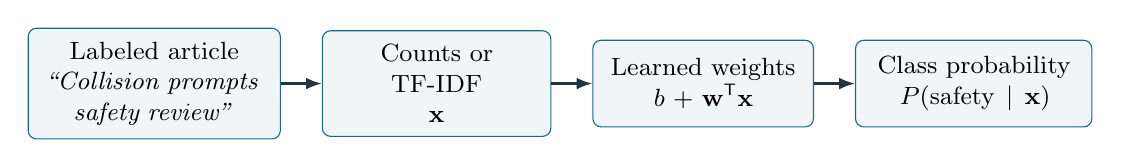
\begin{tikzpicture}[node distance=0.52cm]
\node[flowbox,text width=2.85cm] (text) {Labeled article\\\emph{``Collision prompts safety review''}};
\node[flowbox,text width=2.55cm,right=of text] (features) {Counts or TF-IDF\\$\mathbf{x}$};
\node[flowbox,text width=2.45cm,right=of features] (score) {Learned weights\\$b+\mathbf{w}^{\mathsf T}\mathbf{x}$};
\node[flowbox,text width=2.65cm,right=of score] (prob) {Class probability\\$P(\text{safety}\mid\mathbf{x})$};
\draw[flowarrow] (text) -- (features);
\draw[flowarrow] (features) -- (score);
\draw[flowarrow] (score) -- (prob);
\end{tikzpicture}
\captionof{figure}{Original teaching schematic of text classification, based on the feature-to-prediction descriptions of \textcite{weiss2005} and \textcite{sklearnlogistic}. No values shown are fitted results.}
\end{center}

\subsection*{Example}
\textbf{Illustrative only.} Suppose a class defines \emph{safety incident} versus \emph{policy}. A headline about an autonomous-vehicle collision might receive the safety label, while one about a bill governing road tests might receive the policy label. A story about a bill introduced after a collision could contain both themes; the binary task still requires an explicit labeling rule. Do not present these labels or any predicted probability as results from the group's articles.

\subsection*{Key takeaways}
\begin{itemize}
  \item Logistic regression answers a supervised question: \emph{Which known label fits this article?}
  \item It provides an interpretable baseline, but its bag-of-words or TF-IDF input does not itself represent word order or contextual meaning.
\end{itemize}

\section[LDA: a brief classical overview]{LDA: a brief classical overview \hfill\normalsize\textit{1.5 minutes}}

\subsection*{Sources}
\begin{itemize}
  \item \textcite{blei2003}, the original Latent Dirichlet Allocation paper: documents as mixtures of topics and topics as distributions over words.
  \item \textcite{silgerobinson}, Chapter 6: an accessible two-topic example and interpretation of topic-word and document-topic probabilities.
  \item \textcite{qamar2024}, chapter on text summarization and topic modeling: connection to a classical text-mining workflow.
\end{itemize}

\Needspace{10\baselineskip}
\subsection*{Key concepts and goals}
\begin{itemize}
  \item \textbf{Goal:} find recurring themes in a collection of articles without supplying topic labels for each article.
  \item A \emph{topic} is a distribution over words; an \emph{article} can contain a mixture of topics. The analyst interprets and names topics after fitting \parencite{blei2003,silgerobinson}.
  \item LDA here means \emph{Latent Dirichlet Allocation}. It is a different method from the supervised classifier just introduced.
\end{itemize}

\subsection*{Method}
Start with a document-term representation of the article collection. Choose the number of topics, fit the model, then inspect prominent words for each topic and the topic mixture for each article. The model estimates these distributions together; it does not receive a prewritten list of ``safety'' or ``policy'' topic names \parencite{blei2003,silgerobinson}. Leave the generative process, inference, and topic evaluation to Laura's dedicated LDA segment.

\subsection*{Figures}
\begin{center}
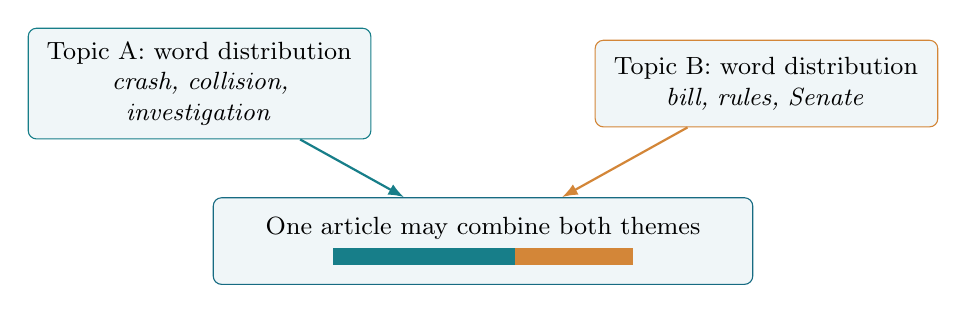
\begin{tikzpicture}
\node[flowbox,draw=topicone,text width=4.0cm] (safety) at (0,0) {Topic A: word distribution\\\emph{crash, collision, investigation}};
\node[flowbox,draw=topictwo,text width=4.0cm] (policy) at (7.2,0) {Topic B: word distribution\\\emph{bill, rules, Senate}};
\node[flowbox,text width=6.5cm] (article) at (3.6,-2.0) {One article may combine both themes\\\rule{0pt}{0.22cm}\textcolor{topicone}{\rule{2.3cm}{0.22cm}}\textcolor{topictwo}{\rule{1.5cm}{0.22cm}}};
\draw[flowarrow,draw=topicone] (safety) -- (article);
\draw[flowarrow,draw=topictwo] (policy) -- (article);
\end{tikzpicture}
\captionof{figure}{Original schematic of topic-word distributions and an article-topic mixture, based on \textcite{blei2003} and \textcite{silgerobinson}. The words and bar lengths are illustrative, not fitted topics or probabilities.}
\end{center}

\subsection*{Example}
\textbf{Illustrative only.} An article about a proposed testing law following an autonomous-vehicle crash could use words associated with both a safety theme and a regulation theme. LDA could assign it a mixture of those discovered topics; this is not a manually assigned class or a claim about the project data.

\subsection*{Key takeaways}
\begin{itemize}
  \item LDA answers an unsupervised question: \emph{What themes recur across these articles?}
  \item Its output is interpretable topic-word and article-topic distributions. \textbf{Handoff to Laura:} how LDA estimates and evaluates them.
\end{itemize}

\clearpage
\section[Word and document embeddings]{Word and document embeddings \hfill\normalsize\textit{4.5 minutes}}

\subsection*{Sources}
\begin{itemize}
  \item \textcite{mikolov2013}, Figure 1: word2vec's CBOW and Skip-gram architectures.
  \item \textcite{le2014}, Figure 2: learned paragraph or document vectors.
  \item \textcite{reimers2019}: later contextual sentence embeddings.
\end{itemize}

\subsection*{Key concepts and goals}
\begin{itemize}
  \item Bag-of-words vectors have many zero vocabulary entries; learned embeddings are shorter, dense vectors \parencite{mikolov2013,le2014}.
  \item \textbf{Goals:} give related words useful nearby vectors and give each article one vector for comparison or downstream learning.
  \item Classic word2vec vectors are \emph{static}: each word has the same vector in different sentences.
\end{itemize}

\subsection*{Method}
CBOW predicts a center word from its neighbors; Skip-gram predicts neighbors from a center word. Both learn vectors for word types \parencite{mikolov2013}. Paragraph Vector learns a document vector that joins local context in word prediction and represents text of varying length \parencite{le2014}. The resulting vectors can be compared or used as model features. This approach differs from extracting embeddings with a pretrained language model.

\subsection*{Figures}
\begin{center}
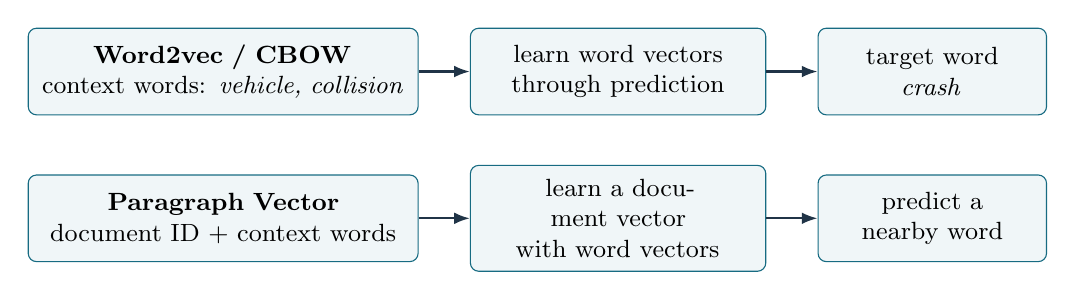
\begin{tikzpicture}[node distance=0.65cm]
\node[flowbox,text width=4.6cm] (context) {\textbf{Word2vec / CBOW}\\context words: \emph{vehicle, collision}};
\node[flowbox,text width=3.4cm,right=of context] (wordvec) {learn word vectors\\through prediction};
\node[flowbox,text width=2.55cm,right=of wordvec] (target) {target word\\\emph{crash}};
\draw[flowarrow] (context) -- (wordvec);
\draw[flowarrow] (wordvec) -- (target);
\node[flowbox,text width=4.6cm,below=0.75cm of context] (doc) {\textbf{Paragraph Vector}\\document ID + context words};
\node[flowbox,text width=3.4cm,right=of doc] (docvec) {learn a document vector\\with word vectors};
\node[flowbox,text width=2.55cm,right=of docvec] (target2) {predict a\\nearby word};
\draw[flowarrow] (doc) -- (docvec);
\draw[flowarrow] (docvec) -- (target2);
\end{tikzpicture}
\captionof{figure}{Simplified adaptations of Figure 1 in \textcite{mikolov2013} (\href{https://arxiv.org/pdf/1301.3781}{original paper}) and Figure 2 in \textcite{le2014} (\href{https://proceedings.mlr.press/v32/le14.pdf}{original paper}). Example words are illustrative.}
\end{center}

\subsection*{Example}
\textbf{Illustrative only.} ``Autonomous-vehicle collision triggers inquiry'' and ``Driverless-car crash prompts investigation'' share few exact words, yet a suitable learned representation could place them near each other. Actual closeness depends on the model; no distance was measured.

\subsection*{Key takeaways}
\begin{itemize}
  \item Embeddings turn words or entire documents into vectors that can support similarity, clustering, or classification.
  \item Earlier word2vec-style word vectors do not change with context; contextual embeddings from pretrained models can.
\end{itemize}

\clearpage
\section[Pretrained language models]{Pretrained language models \hfill\normalsize\textit{4.5 minutes}}

\subsection*{Sources}
\begin{itemize}
  \item \textcite{devlin2019}, especially Figure 1: BERT pretraining followed by task-specific fine-tuning.
  \item \textcite{reimers2019}: Sentence-BERT's fixed-size embeddings for semantic similarity and clustering.
\end{itemize}

\subsection*{Key concepts and goals}
\begin{itemize}
  \item \textbf{Pretraining:} learn general patterns from large amounts of text before the particular class task. \textbf{Reuse:} adapt the model or its representations to a later task \parencite{devlin2019}.
  \item BERT is a Transformer encoder that uses surrounding context on both sides of a token; its masked-token prediction is the pretraining idea to explain aloud \parencite{devlin2019}.
  \item The same written word can receive a different contextual representation in different sentences. Task choice matters: a BERT classifier and a model trained to produce comparable sentence vectors have different outputs \parencite{devlin2019,reimers2019}.
\end{itemize}

\subsection*{Method}
Present a two-stage workflow: pretrain BERT on general text, then add a task head and fine-tune it with labeled articles for classification. For similarity or clustering, use a sentence-embedding model such as Sentence-BERT that is trained to produce comparable fixed-size vectors; do not assume an arbitrary raw BERT output is already a good similarity embedding \parencite{devlin2019,reimers2019}. Mention, in one sentence, that generative language models are another pretrained family that commonly learns to predict the next token; the segment does not cover their architecture or generation behavior.

\subsection*{Figures}
\begin{center}
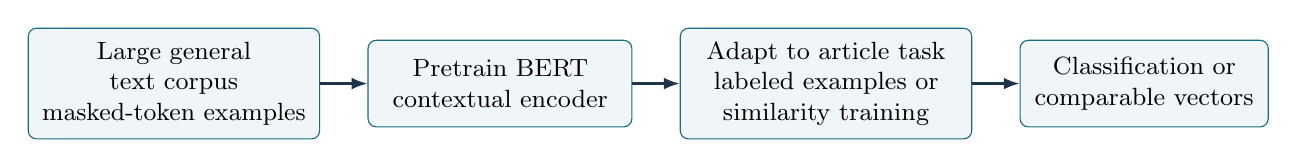
\begin{tikzpicture}[node distance=0.6cm]
\node[flowbox,text width=3.35cm] (corpus) {Large general text corpus\\masked-token examples};
\node[flowbox,text width=3.0cm,right=of corpus] (bert) {Pretrain BERT\\contextual encoder};
\node[flowbox,text width=3.35cm,right=of bert] (adapt) {Adapt to article task\\labeled examples or\\similarity training};
\node[flowbox,text width=2.8cm,right=of adapt] (out) {Classification or\\comparable vectors};
\draw[flowarrow] (corpus) -- (bert);
\draw[flowarrow] (bert) -- (adapt);
\draw[flowarrow] (adapt) -- (out);
\end{tikzpicture}
\captionof{figure}{Simplified adaptation of the pretraining-to-task flow in Figure 1 of \textcite{devlin2019} (\href{https://aclanthology.org/N19-1423.pdf}{original paper}); the similarity-output branch is informed by \textcite{reimers2019} (\href{https://aclanthology.org/D19-1410/}{paper}).}
\end{center}

\subsection*{Example}
\textbf{Illustrative only.} Compare ``The company \emph{charged} the autonomous car overnight'' with ``The company was \emph{charged} after the autonomous-car crash.'' The surrounding words give \emph{charged} different meanings; BERT can produce representations conditioned on each sentence. For the group's news corpus, a task-specific classifier might predict a chosen article label, while a sentence-embedding model could support article similarity or clustering. Neither behavior is claimed as a measured result on the corpus.

\subsection*{Key takeaways}
\begin{itemize}
  \item Pretraining supplies reusable language representations that can be adapted with less task-specific data than training a comparable model from scratch.
  \item Choose an output suited to the goal: class probabilities for classification, comparable document vectors for similarity or clustering.
\end{itemize}

\clearpage
\section*{Comparison and handoff \hfill\normalsize\textit{1 minute}}

\begin{center}
\begin{tabular}{@{}p{0.30\linewidth}p{0.27\linewidth}p{0.32\linewidth}@{}}
\toprule
Method & Main question & Main output \\
\midrule
Logistic regression & Which supplied label? & Class probability / label \\
LDA & What themes recur? & Topic-word and article-topic distributions \\
Embeddings & Which words or articles are similar? & Dense vectors \\
Pretrained language model & How can general language learning help this task? & Contextual features, labels, or task-trained vectors \\
\bottomrule
\end{tabular}
\end{center}

\textbf{Closing line:} ``We have seen what LDA contributes alongside classification and embeddings: interpretable themes without article labels. Laura will now show how LDA finds those themes and how we can judge them.''

\printbibliography[title={References}]

\end{document}
